\documentclass[11pt]{article}

\usepackage[margin=0.75in]{geometry}
\usepackage{graphicx}
\graphicspath{ {images/} }

\title{The title of your project proposal}
\author{
  Jara, Jon\\
  \texttt{jonmigueljara}
  \and
  Shishido, Juan\\
  \texttt{juanshishido}
  \and
  Xu, Wendy\\
  \texttt{berithsu}
}

\bibliographystyle{siam}

\begin{document}
\maketitle

\abstract{
The goal of this research is to analyze brain activities associated with
decision-making. In particular, we draw upon the experiment of mixed gambles to
investigate the relationship between neural and behavioral loss aversion. The
relationships are observed by neural activities, measured as fMRI data, when
subjects are exposed to gambles. Our project attempts to apply linear
regression and multi-voxel pattern analysis to study loss-and-gain sensitivity
levels inside the brain.
}

\section{Introduction}

Our research idea is based on the 2007 paper The Neural Basis of
Loss Aversion in Decision-Making Under Risk, written by Sabrina M. Tom, Craig
R. Fox, Christopher Trepel, and Russell A. Poldrack\cite{tom}. Our goal is to
reproduce the major part of the paper with possible simplifications and also
develop some original analysis on the same data.

A significant portion of the paper is devoted to analyzing neural
indicators of loss aversion and correlating that neural loss aversion to
behavioral loss aversion. Test subjects are presented with gambles with equal
chances of winning and losing and different amounts of money to gain and lose.
These gamble offers and the subject's decision of whether or not to accept the
gamble are recorded, as well as the subject's neural activities during the
tasks. Behavioral risk aversion is measured through modeling the participant's
decision on the amount of proposed gain and loss of the gambles. On the other
hand, neural risk aversion is measured through modeling the participant's fMRI
data on the amount of proposed gain and loss of the gambles. The researchers
find that behavioral loss aversion is statistically correlated with neural risk
aversion. Another finding is that that some areas of the brain are particularly
sensitive to both gains and losses, exhibiting increasing activity as potential
gains increase and decreasing activity as potential losses increase. Neural
activities in these areas can reasonably be used to predict behavioral loss
aversion.

The main approach used by the researchers is called the ``matrix analysis.''
The gain/loss matrix, from where gambles are randomly drawn and displayed to
the experiment subject, is collapsed from a 16 x 16 into a 4 x 4 matrix and
trials for all subjects and runs are grouped according to this smaller matrix,
resulting in 16 separate conditions. Separate estimation of the evoked response
for each of these conditions enables the comparison between ``good'' versus
``bad'' gambles. Another separate approach is the ``parametric analysis,''
where all the trials are modeled by orthogonal parametric regressors
representing the size the potential gain, the size of the potential loss, and
the Euclidean distance of the gain and loss combination from the diagonal of
the gain/loss matrix. Both methods are carried out by time-series analysis
using FILM (FMRIB’s Improved Linear Model).

We will reproduce this part of the paper using mostly linear regression and
logistic models and evaluate our results against the paper's results as well as
using error analysis. We will also visualize our research results consistently
with 2-D and possibly 3-D graphs. We would also like to experiment with
multi-voxel pattern analysis on the fMRI data, which helps detect patterns of
brain activity by jointly analyzing multiple voxels at the same time. 

\section{Data}

\subsection{Description}

The data set includes 3 sample runs for each subject, with 16 subjects in
total. The subjects consist of 9 females and 7 males. For each run, the subject
is presented with a series of gambles with different combinations of gains and
losses, each combination randomly drawn from a gain/loss matrix of size 16 x
16. For the purpose of analysis, the data are collapsed into a 4 x 4 matrix.
The subject's fMRI data generated during the tasks is available for each run.

The typical brain image consists of 64 x 64 voxels for each brain slice and 34
slices in total. Repetition time (TR) is 2 seconds. Two volumes are discarded
at the beginning of each run.

\subsection{Acquiring}

A primary goal of ours is to ensure that individuals who wish to replicate or
improve upon our work can easily do so. To that end, in terms of data access,
we have created a bash script that fetches the data from www.openfmri.org and
untars it. It runs only if the data directory doesn't already exist. The script
also downloads the checksums and we've written a Python script to check that
the hashes match. We will incorporate the Python script in the Makefile for
downloading the data.

\section{Methods}

\subsection{Preprocessing}

We are considering several preprocessing techniques to use on our data.

\subsubsection{Smoothing}

After initial plots, we observed that the data was noisy. Smoothing in space
reduces the noise by averaging data---in this case, voxels---with its
neighbors, while preserving signal. This is typically done using a Gaussian
function. The selected width of the distribution determines how much the data
are smoothed.

There are several benefits related to smoothing. Below, we list the ones that
are relevant for our analysis.

\begin{itemize}
  \item increased sensitivity
  \item making the error distribution normal
\end{itemize}

We are also aware of the following disadvantages.

\begin{itemize}
  \item{reduced spatial resolution}
  \item{edge artifacts}
\end{itemize}

Typically, for single-subject analyses, a width of 4 mm is used. This
information came from the Brain Voyager website\cite{bvsmoothing}.

The first step we took in pre-processing the blood-oxygen-level dependent
(BOLD) image data was to smooth the BOLD data using a Gaussian filter by two
standard deviations in all three spatial dimensions. Figure
~\ref{fig:smoothing-before} and Figure ~\ref{fig:smoothing-after} show how
smoothing vastly improves the interpretability of the single brain images (note
that these images were not the final plots used in analysis, these are just to
show how images looked before and after smoothing).

\begin{figure}[h]
\caption{Before Smoothing}
\centering
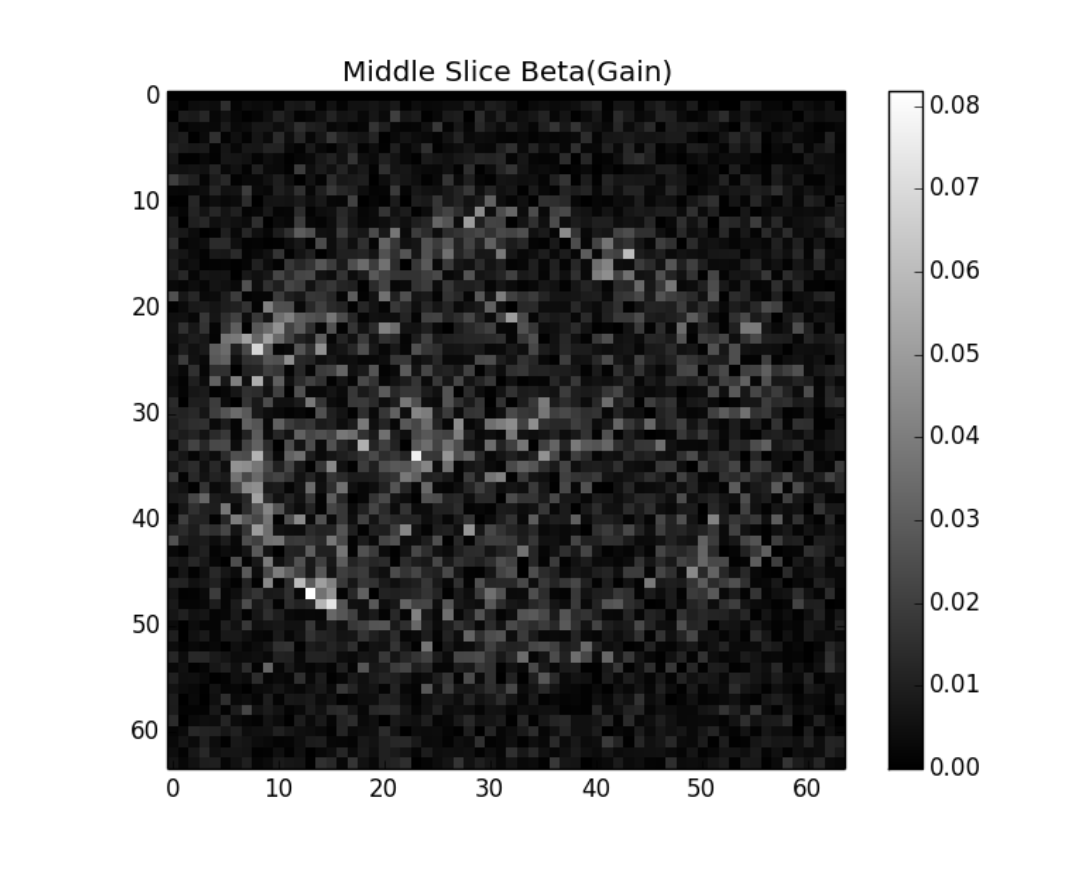
\includegraphics[width=0.5\textwidth]{smoothing-before.png}
\label{fig:smoothing-before}
\end{figure}

\begin{figure}[h]
\caption{After Smoothing}
\centering
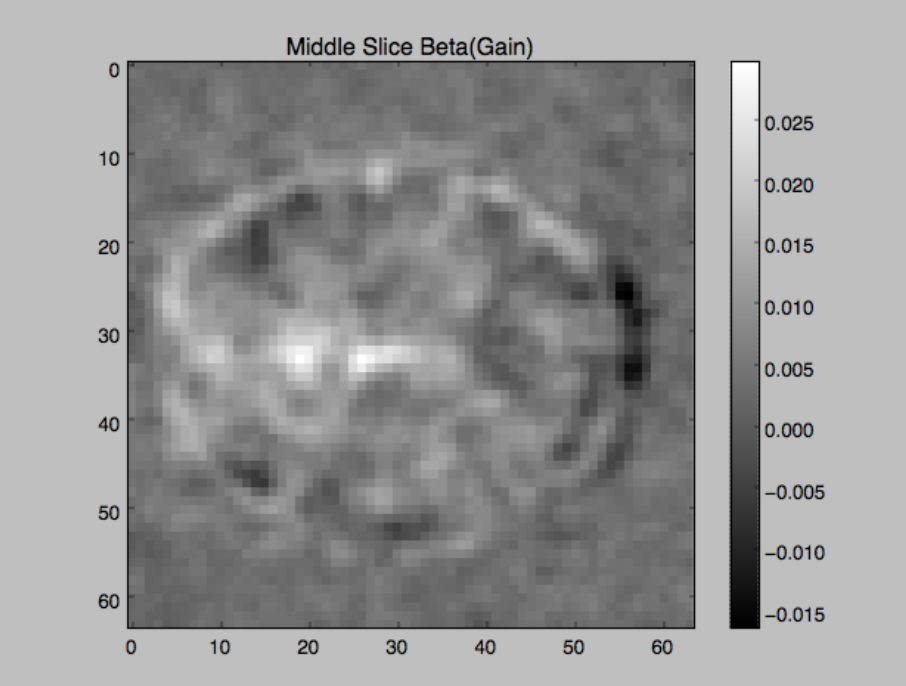
\includegraphics[width=0.5\textwidth]{smoothing-after.png}
\label{fig:smoothing-after}
\end{figure}

\subsubsection{Outliers}

The next step was to use  RMS of the BOLD fMRI signal to locate and remove
outliers to further remove noise from the data. We found that the number of
outlying  volumes varied greatly from subject to subject and from subject to
run with some runs having as many as 100 volumes removed and as little as 0. We
plotted RMS values with outliers marked with red markers (similar to what we
did in homework 2). Figure ~\ref{fig:outliers-1-1} and Figure
~\ref{fig:outliers-9-3} are two examples of how we identified outliers.

\begin{figure}[h]
\caption{Subject 1, Run 1}
\centering
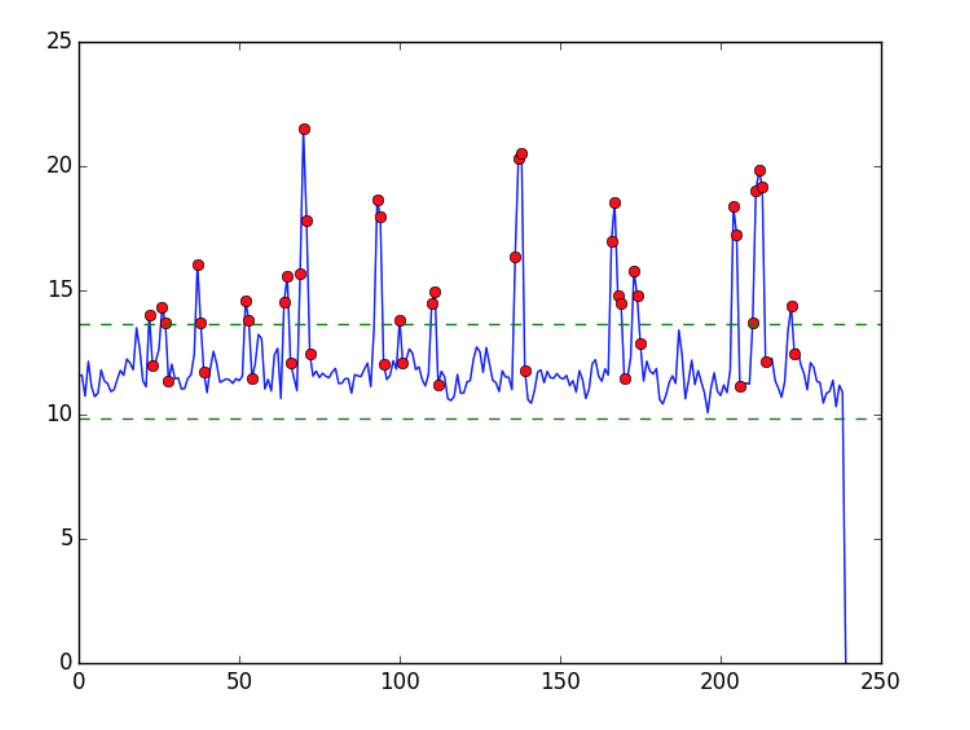
\includegraphics[width=0.5\textwidth]{outliers-1-1.png}
\label{fig:outliers-1-1}
\end{figure}

\begin{figure}[h]
\caption{Subject 9, Run 3}
\centering
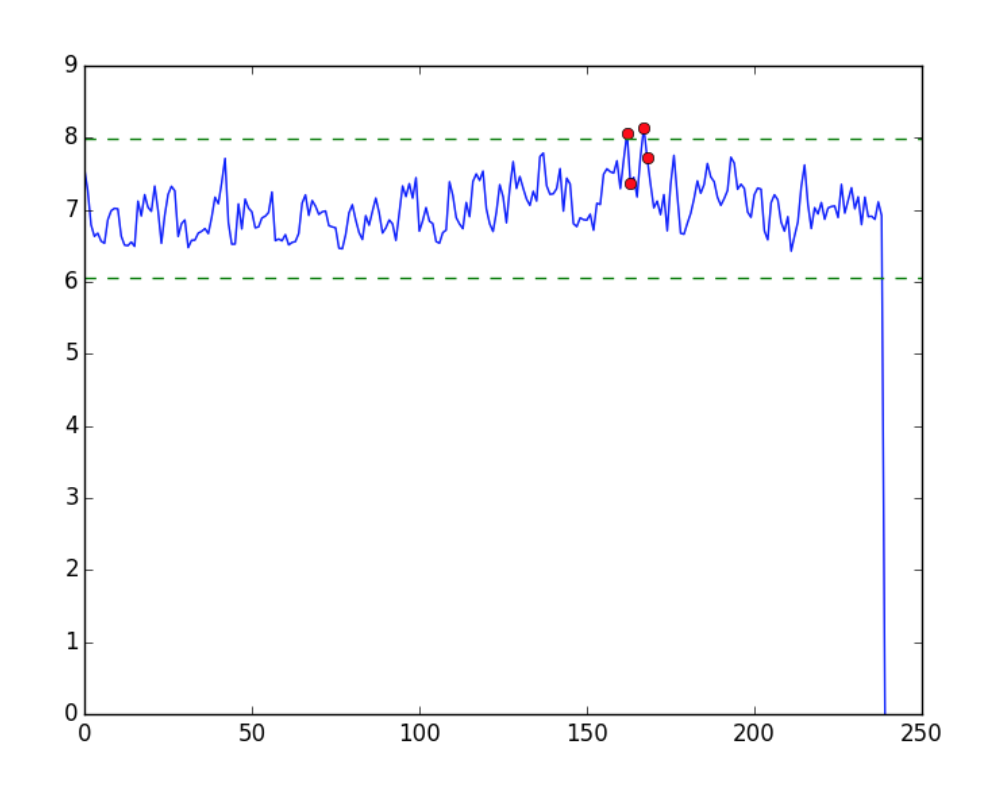
\includegraphics[width=0.5\textwidth]{outliers-9-3.png}
\label{fig:outliers-9-3}
\end{figure}

\subsection{Analysis and Results}

In their primary analysis, the researchers build statistical models separately
for each imaging run and create regressors by convolving a delta function
representing trial onset times with a canonical hemodynamic response function.
Similarly, in our research, we will model each run independently and convolve
predictors of interest with a gamma hemodynamic response. We will build linear
regression models for each run using these convolved regressors and
specifically look at the coefficients of those representing gains and losses.
Then we will visualize the coefficients for different slices of the brain to
discover patterns. We also plan on exploring multi-pattern voxel analysis. Both
of these are described in greater detail, below.

\subsubsection{Primary}

\textbf{Behavioral Data}

At first ,we attempted to find correlations between behavioral and neural risk
aversion, but this might have been too ambitious of a goal. We simplified our
goal by attempting to find areas of the brain that are sensitive to potential
loss and potential gain. The result would lead to which parts of the brain are
responsible for making risky decision. The first step is to fit a logistic
regression on the behavioral data using a simple linear regression. We used a
combination of pandas and Statsmodels to fit a logistic regression model on the
first subject and all the runs combined. Python modules were used rather than R
packages in order to keep the whole project in the same language and for
reproducibility. The logistic regression was modeled in this manner:

\[ logit(p) = \beta_0 + \beta_1 X_{gain} + \beta_2 X_{loss} + \epsilon \] 

With gain and loss values beings the 2 regressors in the regression. Subject 1
had a gain to loss ratio of 2.33, which was inline with gain to loss ratio
cited by other sources in the paper (around 2.0). The paper was not specific in
how they dealt with multiple runs per subject but we decided that it would be
sound to average all the runs for each patient and then average all the
subjects.

\textbf{BOLD Data}

Next was our analysis of the neural image data. The goal of this section is
find parts of the brain that are most sensitive to potential gains and
potential loss. After running our preprocessing scripts on all the image data,
we fitted a linear model for every subject and every run. The design matrix for
each linear fitted consisted for 240 rows for each time course with a column of
1’s (for the intercept), the general task onset times, the size of gain, and
the size of loss (all convolved). Also, linear drift and quadratic lift terms
were added to reduce noise from movement. Figure ~\ref{fig:design-matrix}
shows an example of design matrix for subject 1, run 1.

\begin{figure}[h]
\caption{Design Matrix}
\centering
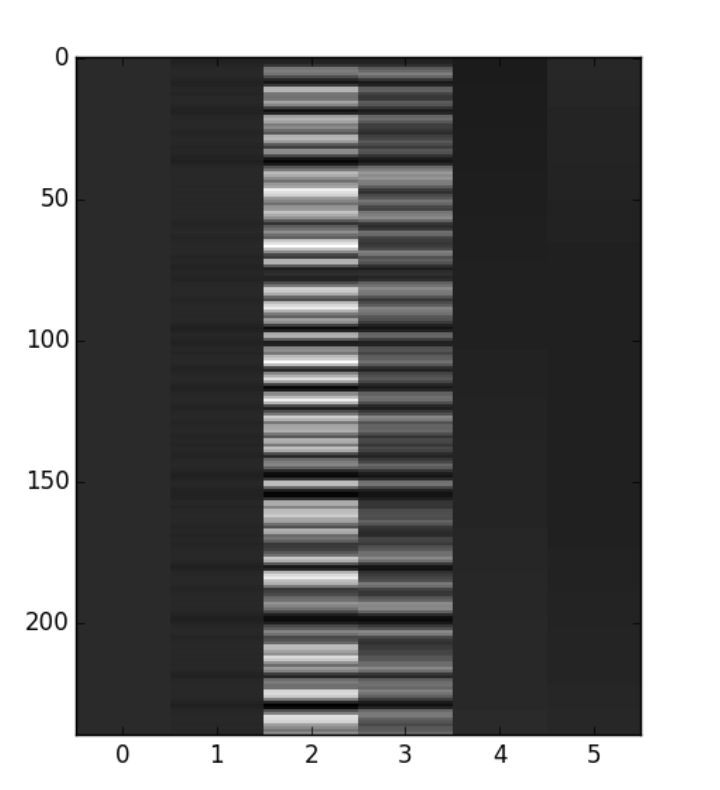
\includegraphics[width=0.5\textwidth]{design-matrix.png}
\label{fig:design-matrix}
\end{figure}

The paper did not specify how all the subjects and all the runs were
collaborated for analysis but we decided to run the linear model for each run
and each subject, average the coefficients for each run for each subject, then
average the coefficients for each subjects. The result is an ``average brain''
that combines the images for all subjects and runs that provide mean
estimations for each coefficient in the regression. Figure ~\ref{fig:gain} and
Figure ~\ref{fig:loss} show the gain and loss responses, respectively.

\begin{figure}[h]
\caption{Gain}
\centering
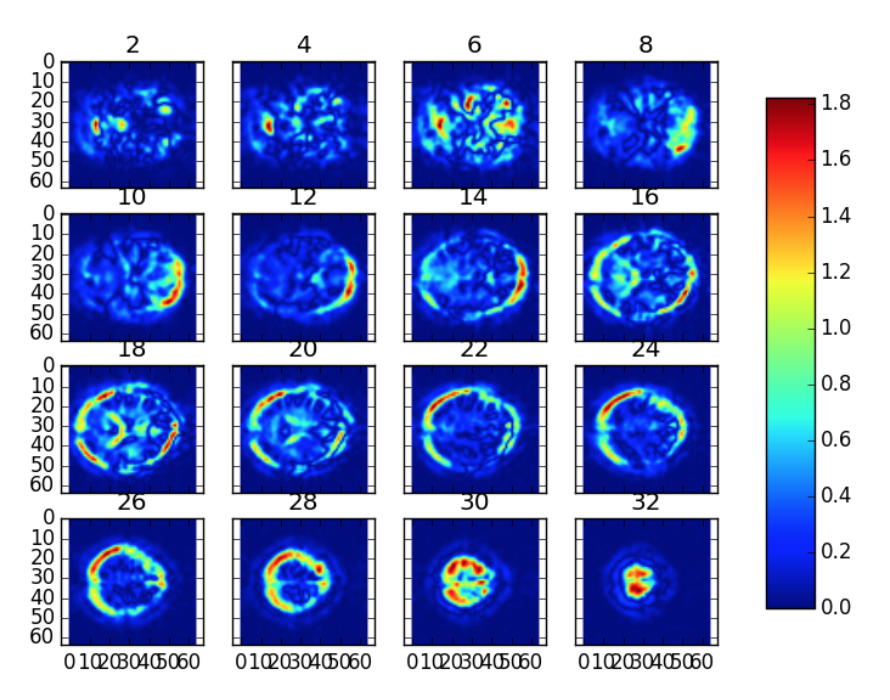
\includegraphics[width=0.5\textwidth]{gain.png}
\label{fig:gain}
\end{figure}

\begin{figure}[h]
\caption{Loss}
\centering
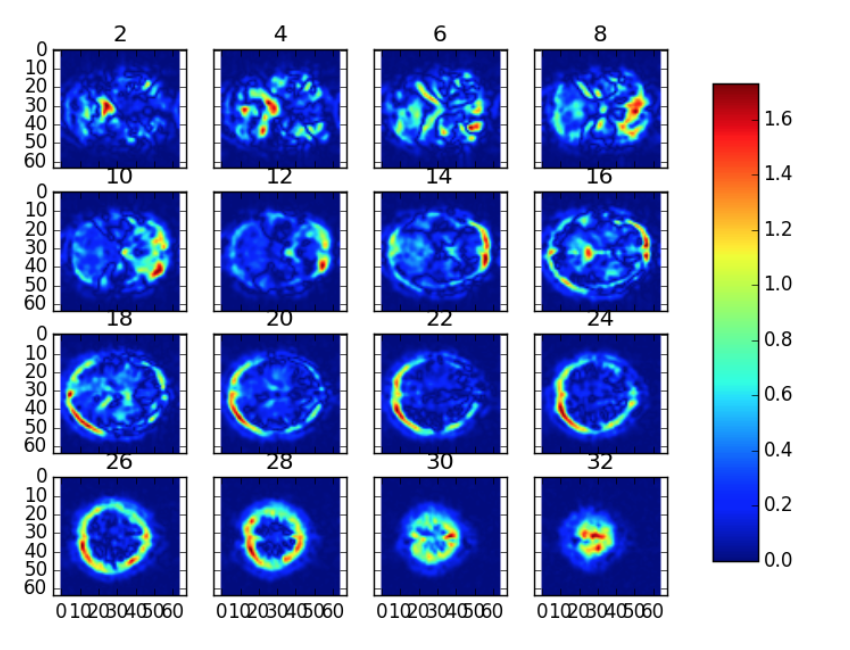
\includegraphics[width=0.5\textwidth]{loss.png}
\label{fig:loss}
\end{figure}

We plotted 16 central slices of the average brain to observe beta coefficient
values and compare between gain or loss. Interestingly, the areas of activation
tend to be around the same areas for beta and loss coefficients. Obvious issues
are the ``edgeyness'' of the plots, in which the edges of the brain images are
being activated but are more likely due to noise due to motion during scans.
Also, the values of the coefficients show that the gain and loss regressors are
similar in magnitude. However, before adding the linear and quadratic drift
term, a gap between both magnitude and volume of brain activity is more
apparent. Figure ~\ref{fig:gain-before-drift} and Figure
~\ref{fig:loss-before-drift} show the gain and loss responses before drift.

\begin{figure}[h]
\caption{Gain Before Drift}
\centering
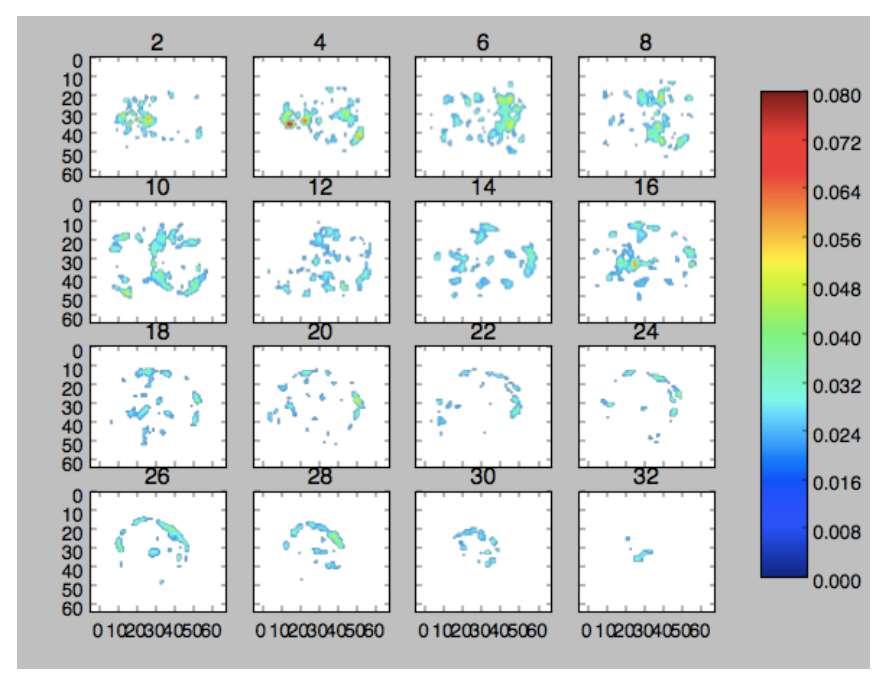
\includegraphics[width=0.5\textwidth]{gain-before-drift.png}
\label{fig:gain-before-drift}
\end{figure}

\begin{figure}[h]
\caption{Loss Before Drift}
\centering
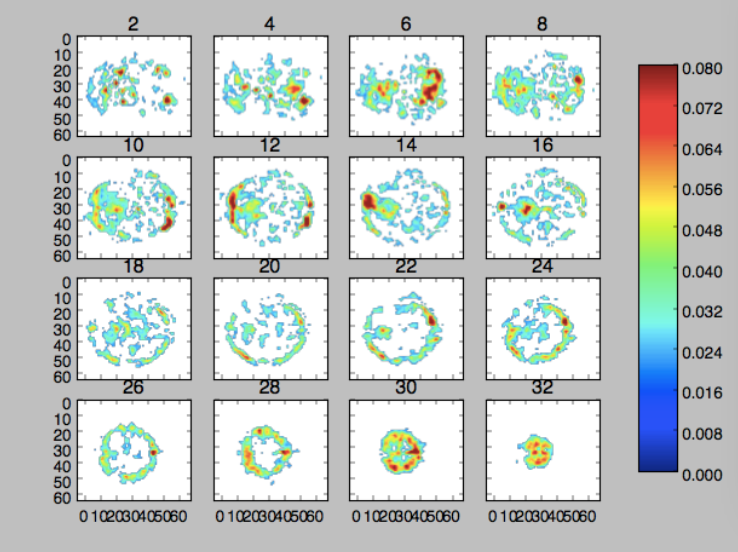
\includegraphics[width=0.5\textwidth]{loss-before-drift.png}
\label{fig:loss-before-drift}
\end{figure}

In the end, noise proved to be our biggest obstacle for analysis and prevent us
from making any valid inferences from the brain images. We do have a rough idea
of where the signals are potentially happening, but we cannot decipher between
the signals due to noise and actual activity. A major component missing from
the analysis is an investigation of the PCA of data to find artefacts that
could be causing noise. For example, the PCA analysis would most likely remove
the right chunk of activity in slices 18 to 24 that is very likely to be an
artifact. It is clear that more work is needed to remove as much noise as
possible from the estimated coefficients.

\subsubsection{Secondary}

As part of our secondary analysis, we are investigating whether it is possible
to use multi-voxel pattern analysis (MVPA) on our data. Norman, Polyn, Detre,
and Haxby note that MVPA allows researchers to analyze \textit{vectors} of
voxel activity values instead of individual ones\cite{norman}. There is greater
sentivity with this focus on distributed patterns of activity, making it easier
to detect differences between conditions\cite{bvmvpa}. Typically, linear
classifiers, such as Gaussian Naive Bayes or linear support vector machines,
are used in MVPA analyses\cite{norman}. The features correspond to the brain
activity and the labels to the cognitive state. MVPA also provides the ability
to correlate subject-level classifier estimates across multiple
trials\cite{norman}.

MVPA uses groups of voxels to classify experimental conditions. In our case,
these conditions are gain and loss gambles (or responses to those gambles).
Groups of voxels are typically defined as ``spheres'' from some ``center''
index. The set the default sphere radius to 1. However, it can be of any
arbitrary size, so long as the \textit{diameter} is not larger than the
smallest dimension of the image.

As an example, a sphere with radius 1 will be made up of 27 voxels---9
for each of the three vertical (\(z\)) slices. From the center voxel, the
sphere is made up of the eight surrounding voxels on its plane as well as the
9 corresponding voxels above and below it. While we call the group of voxels a
``sphere,'' we are actually working with cubes.

Because we may not know, a priori, what regions of interest (ROI) in the brain
contain the signals we're interested in, we use a process called
``searchlight'' that fits a classifier on (almost) every sphere across the
entire brain, one at a time. We exclude spheres with center values equal to
zero.

For each subject and each run, the data include 240 time slices. We don't use
all of these for classification. Rather, we restrict the samples (rows) to
those where the time course is equal to one. In other words, the slices where a
gamble occurred. About 85 of the 240 time slices corresponded to gambles.

``Cross-validation'' is a model validation practice to help determine how well
a model will generalize to new, unseen data. It can help avoid the problem of
``overfitting,'' which is the scenario where the model is only good at
predicting the data is was trained (or fit) on. In other words, cases where a
model is not generalizable. During this process, only part of the data is used
to train the model, which is then used to predict the other part. This split is
done randomly. In addition, because we have the access to the ground truth
values, we are able to determine a prediction accuracy. For MVPA, the
cross-validation approach is called ``leave block out.'' This uses groups of
runs to classify other runs.

Once we have our classification accuracy scores, we assign those to the sphere
centers. While prediction accuracy does not necessarily tell us about
activation, ``If this performance of the classifier is significantly above
chance, one concludes that the [blood-oxygen-level dependent] BOLD responses
contain information about the classified states, and infers that the brain area
where the signals originated is somehow involved in the neural representation
of these states''\cite{schreiber2013statistical}.

For classification, the MVPA function we wrote could take any Scikit-Learn
classifier. We experimented with both logistic regression and the random forest
classifier, but ended up choosing the former. Figure ~\ref{fig:mvpa} shows the
MVPA results for a middle slice of subject 1.

\begin{figure}[h]
\caption{MVPA}
\centering
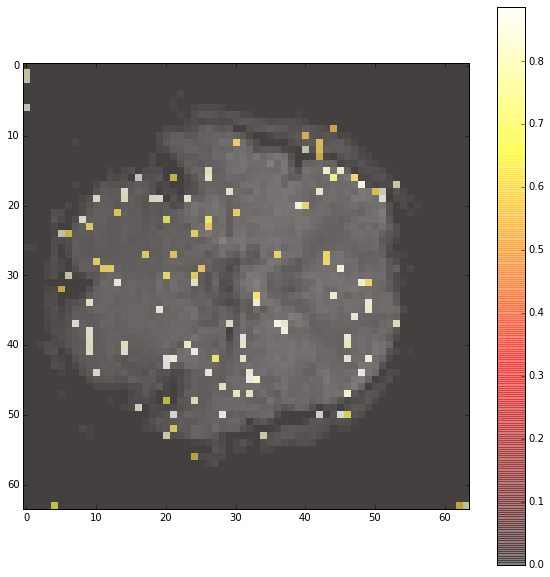
\includegraphics[width=0.5\textwidth]{mvpa.png}
\label{fig:mvpa}
\end{figure}

It's not clear that we're detecting anything substantial. There are two main
reasons for this. First, we used the time course data as the labels we
predicted and these labels were not time-corrected. Second, the gain and loss
gambles were not balanced in the data. That is, there were many more gain
gambles than loss ones. This makes it difficult to interpret accuracy since
prediciting the major class for all samples was often a good strategy.

We would have liked to have the opportunity to correct both of these issues. We
believe the MVPA could be useful for this analysis.

\subsection{Tools}

We have identified several Python packages we will use for our analysis.

\begin{itemize}
  \item{NumPy}
  \item{pandas}
  \item{Nibabel}
  \item{Statsmodels}
  \item{Scikit-Learn}
  \item{Matplotlib}
  \item{Seaborn}
\end{itemize}

\section{Discussion}

\subsection{Challenges}

Many of our issues so far have stemmed from the open ended nature of the
assignment, resulting in less direction than we are used to. This, combined
with the new git workflow, has given us some problems that we are working on
overcoming with a more rigid implementation plan that gives everyone a role.
We are currently using the workflow as best we can, but will be adding many
more Git issues in the coming days in order to better assign work and
facilitate multiple pull requests without merge conflicts. We're having good
success with Python code when we have a good implementation plan. However, a
good deal of our codebase deals with fMRI analysis that we haven't had much
experience working with. This has led to difficulty writing effective tests,
tests that can inspire full confidence in our implementations. We're working on
keeping them simple, using basic modular functions on small datasets to ensure
adequate coverage.

\subsubsection{Team}

We have been working well as a team, and most of our problems are simply
efficiency related. Each of us has applicable skills, we're just trying to get
them all streamlined. This is coming together through the workflow, mainly in
GitHub issues. This allows each of us to work on a different part of the
project at the same time. We have had trouble getting everyone together at the
same time due to erratic schedules, but have been overcoming this using the
workflow.

\subsection{Class Concepts}

We think that we could have used practice in more advanced fMRI analysis
techniques. We've been having some problems with preprocessing, which involves
much more detailed work than we thought. We're looking into some extra Python
libraries to help sort out some advanced preprocessing techniques, smoothing
out confounding variables like respiration and heartbeat. The workflow has been
the most helpful focus, but we think we could have used even more practice.
Because the workflow facilitates efficient team work, we would have liked to
have seen some more group exercises or homework aimed at perfecting the
process.

\bibliography{report}

\end{document}
